\question A 54 kg astronaut takes a 10 kg fire extinguisher with her outside to put out a small fire. She sprays the extinguisher for 2 seconds while it exerts a constant force of 50 N. The force pushes the astronaut (who is still carrying the fire extinguisher) backward and away from the ship (Figure 1).
\begin{figure}[ht!]
	\centering
	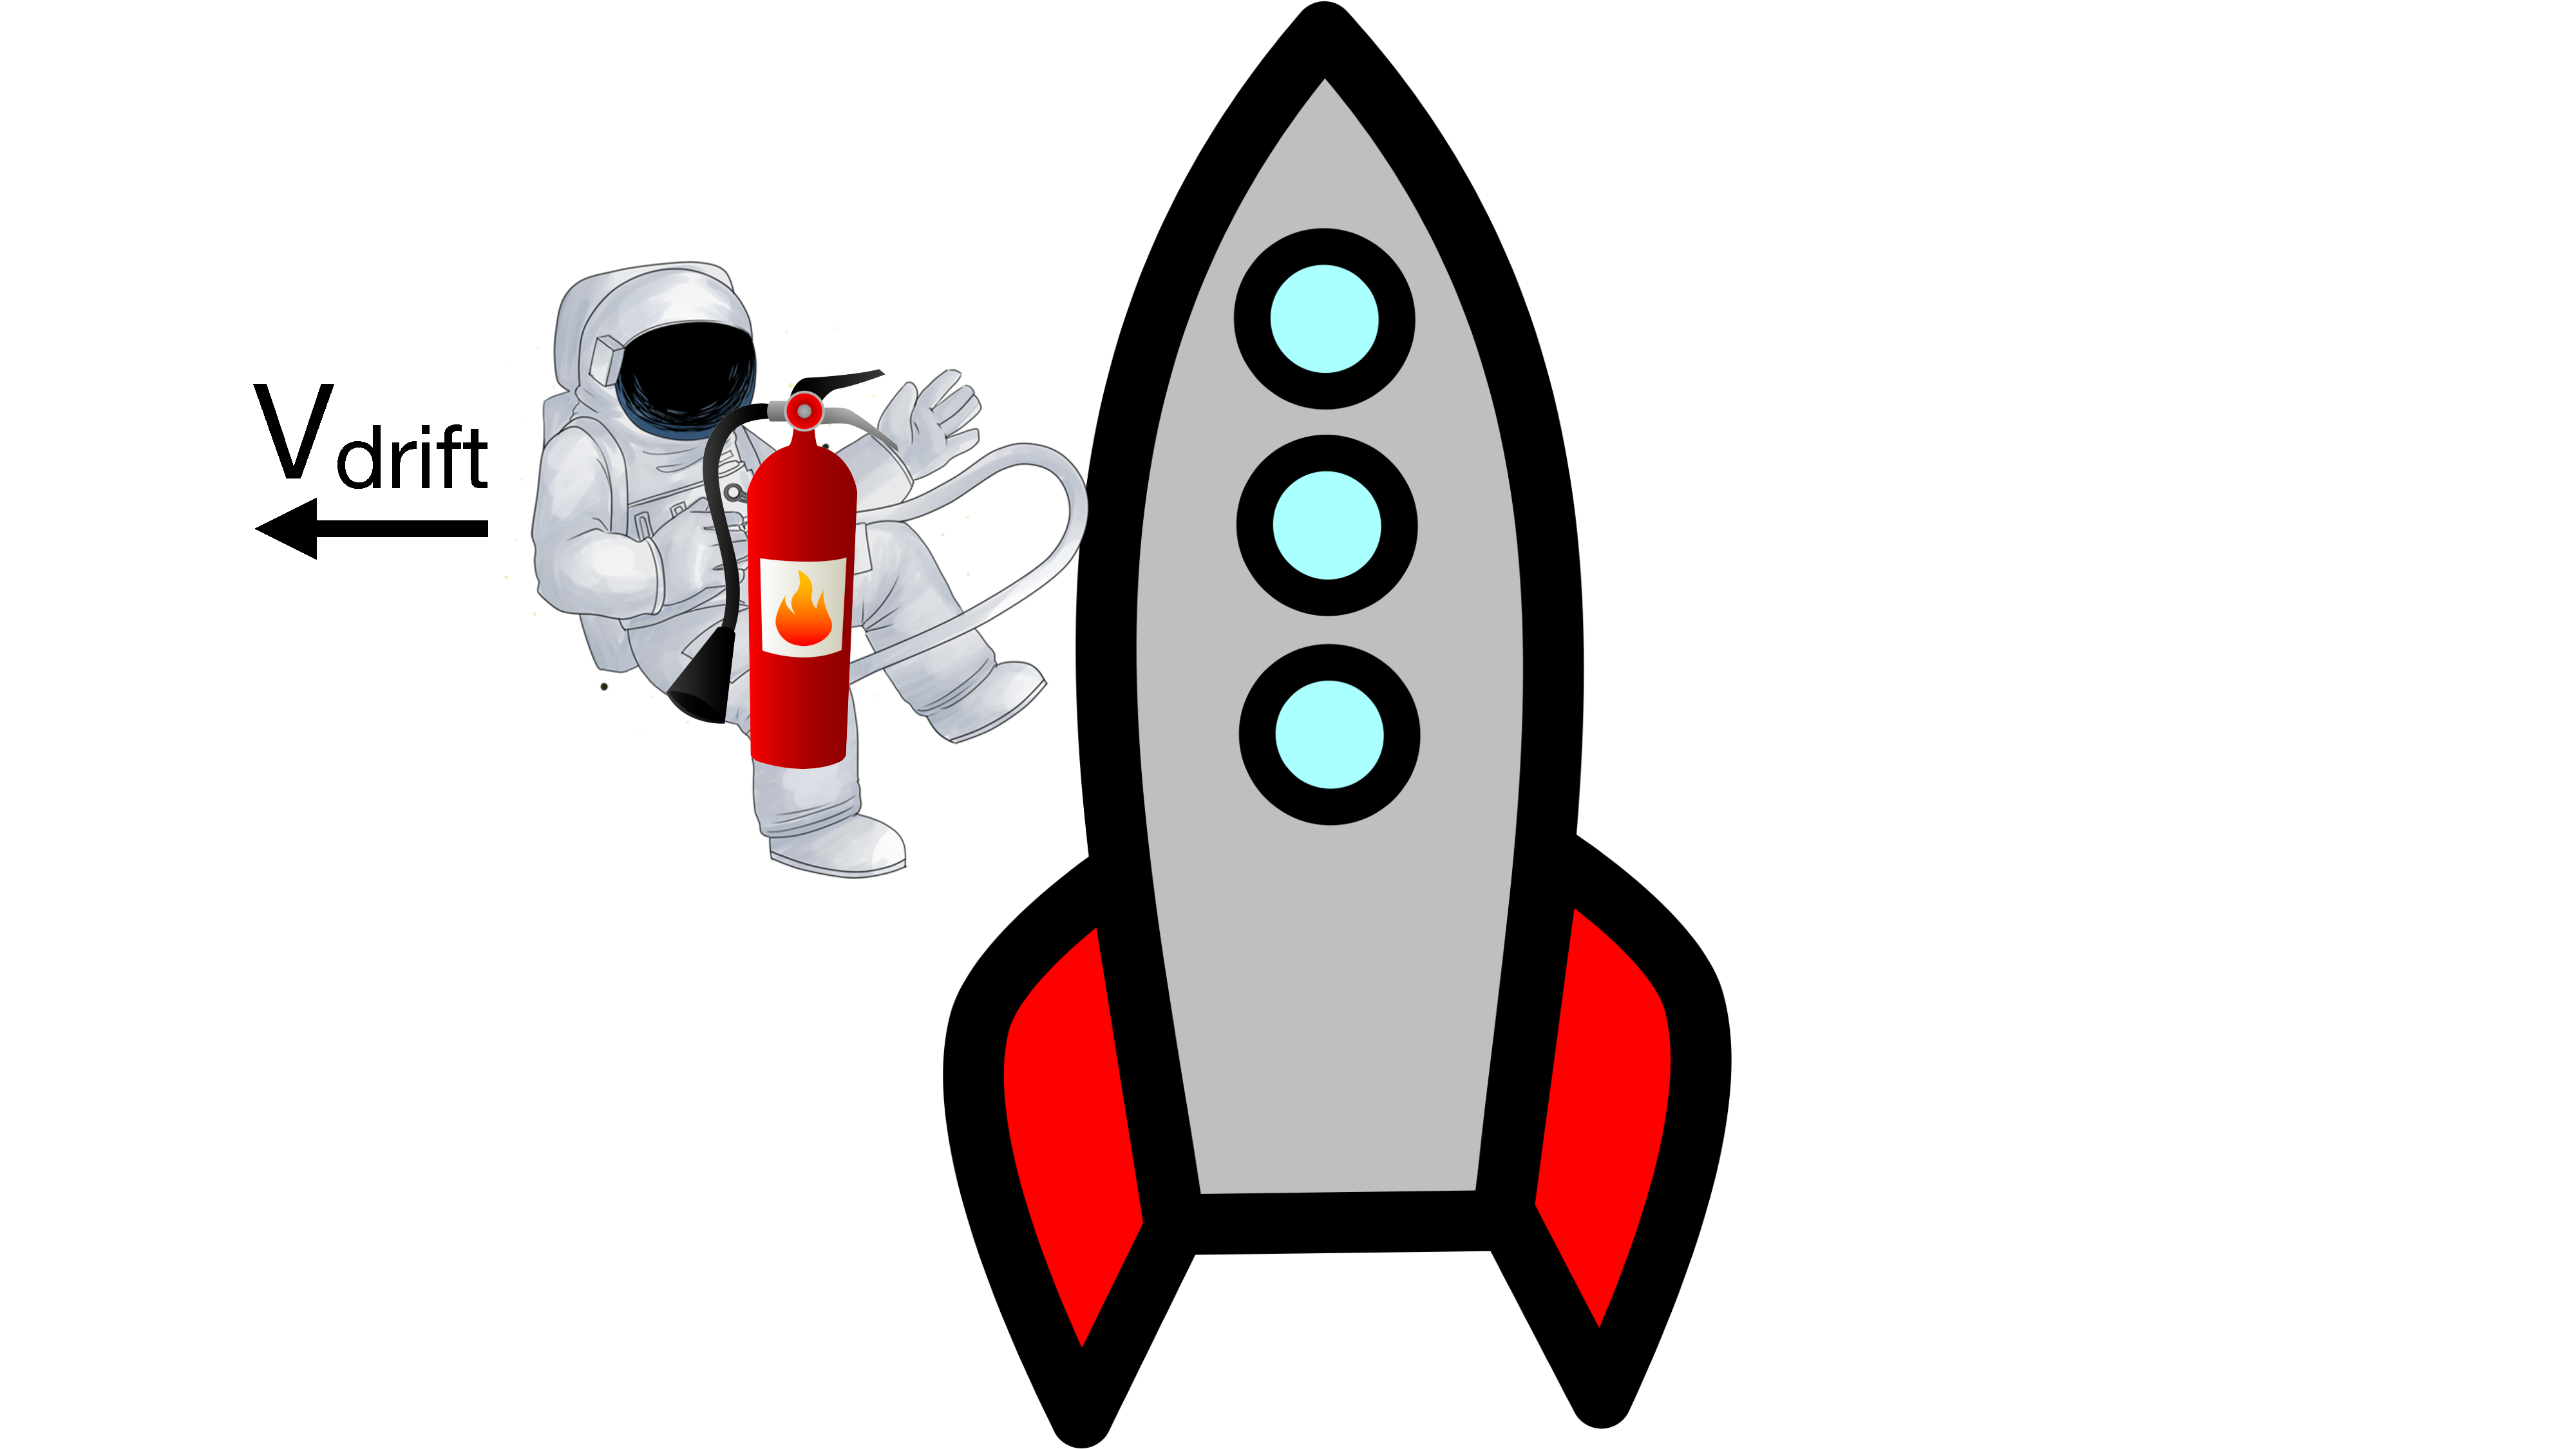
\includegraphics[width=5cm]{astronaut_extinguisher1.pdf}
	\caption{Astronaut and extinguisher drift backward}
\end{figure}
\begin{parts}
\part[10] Assuming that the mass of the fire extinguisher hasn't changed, with what speed are the astronaut and extinguisher drifting away from the ship?
\vspace{5cm}
\part[10] In an attempt to change her velocity to move back toward the ship, the astronaut throws the 10 kg extinguisher backwards so that it moves at a speed of 15 m/s. After throwing the extinguisher, what direction is her velocity (away from or toward the ship)? What is her speed?

\begin{figure}[ht!]
	\centering
	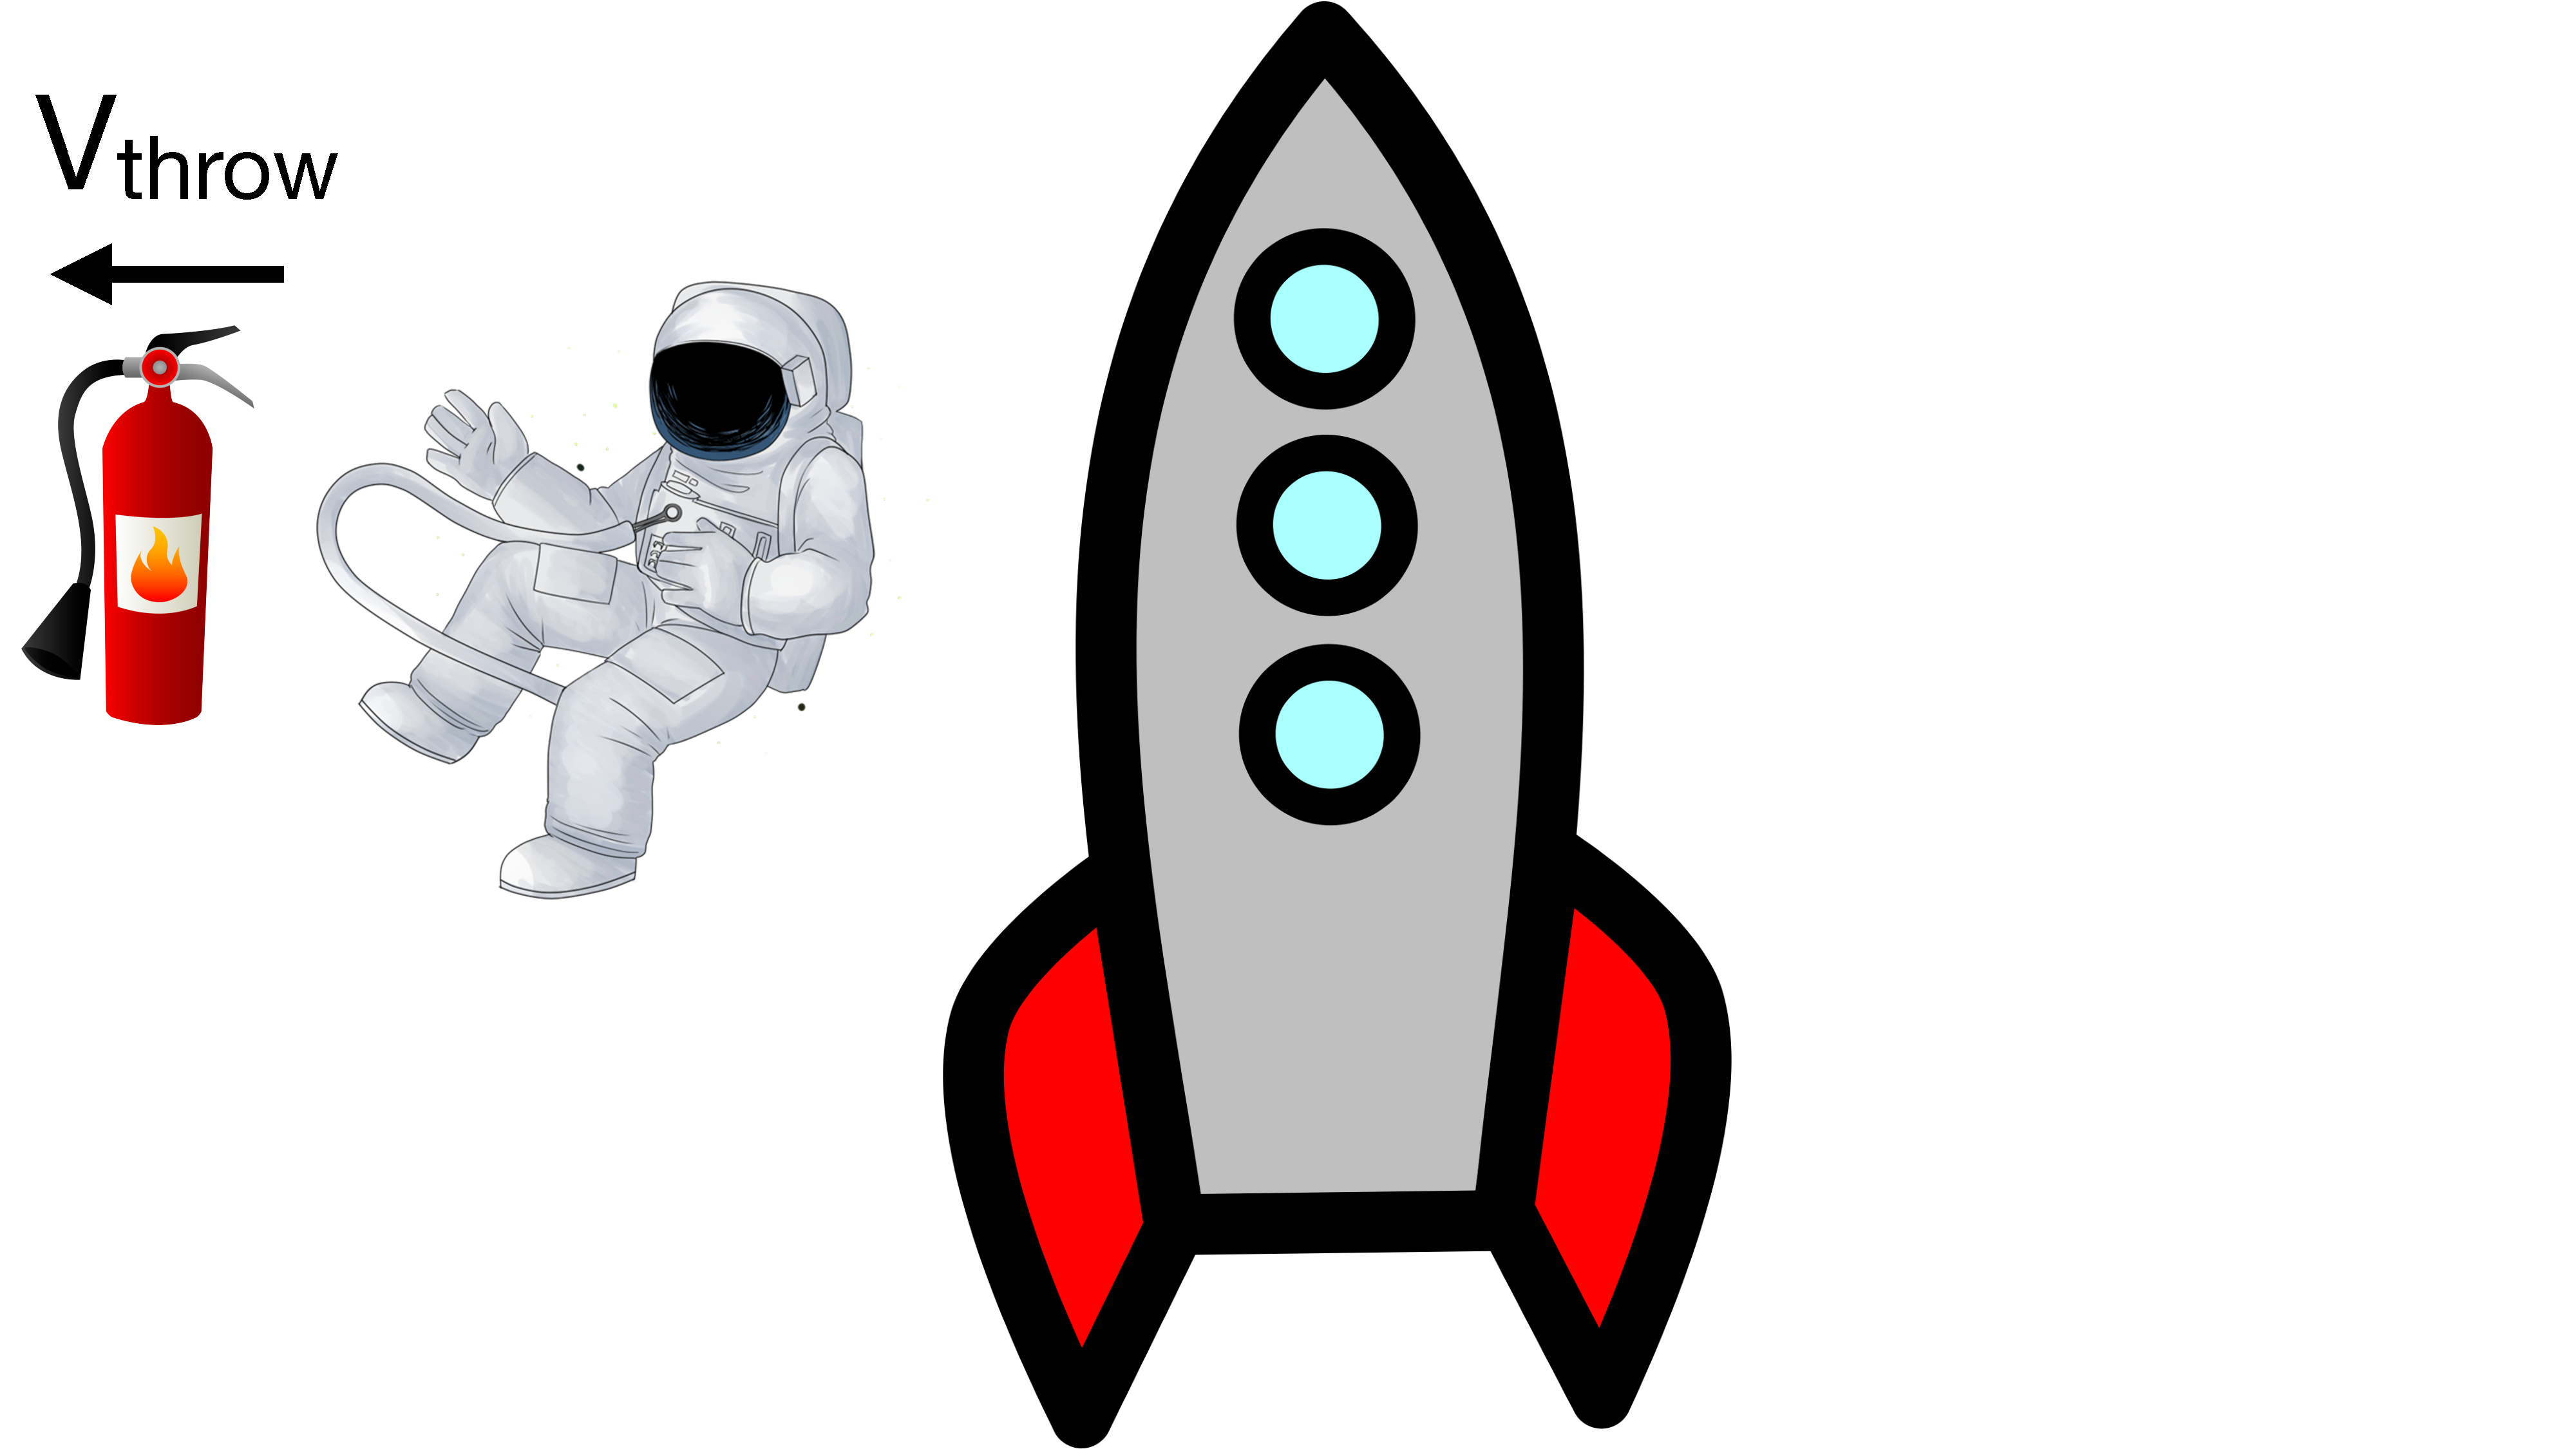
\includegraphics[width=5cm]{astronaut_extinguisher2.pdf}
	\caption{Astronaut throws extinguisher backward}
\end{figure}
\end{parts}